\begin{document}
\chapter*{Resume Oracle APEX}
\section*{Pembuatan Aplikasi Oracle Apex}
\begin{enumerate}

\item[1]Pergi ke Website Oracle APEX, https://apex.oracle.com, lalu klik Get Start For Free.

\begin{figure}[!htbp]
    \begin{center}
    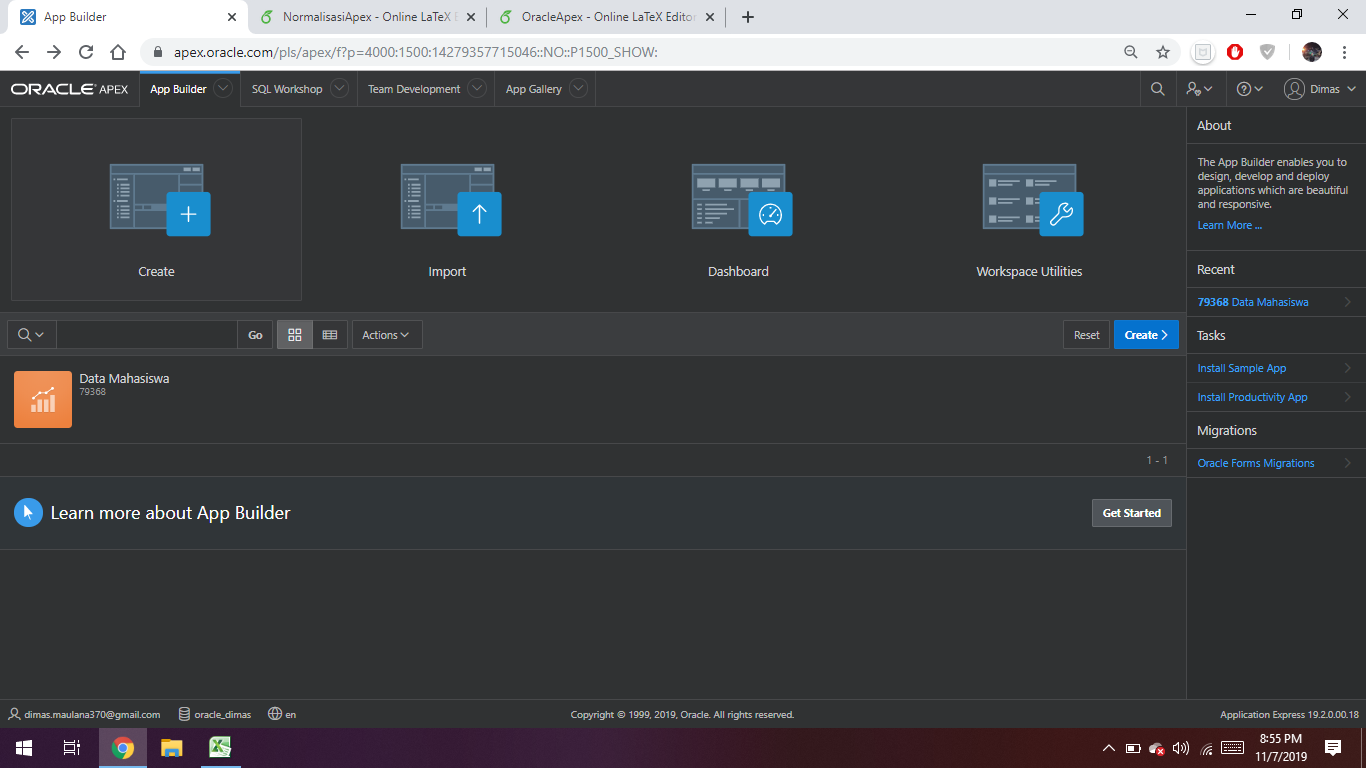
\includegraphics[scale=0.2]{apex/apex1.png}
    \caption{\textit{cara 1}}
    \end{center}   
    \end{figure}
    
\begin{figure}[!htbp]
\item[2]Pilih Request a Free Worksace.

    \begin{center}
    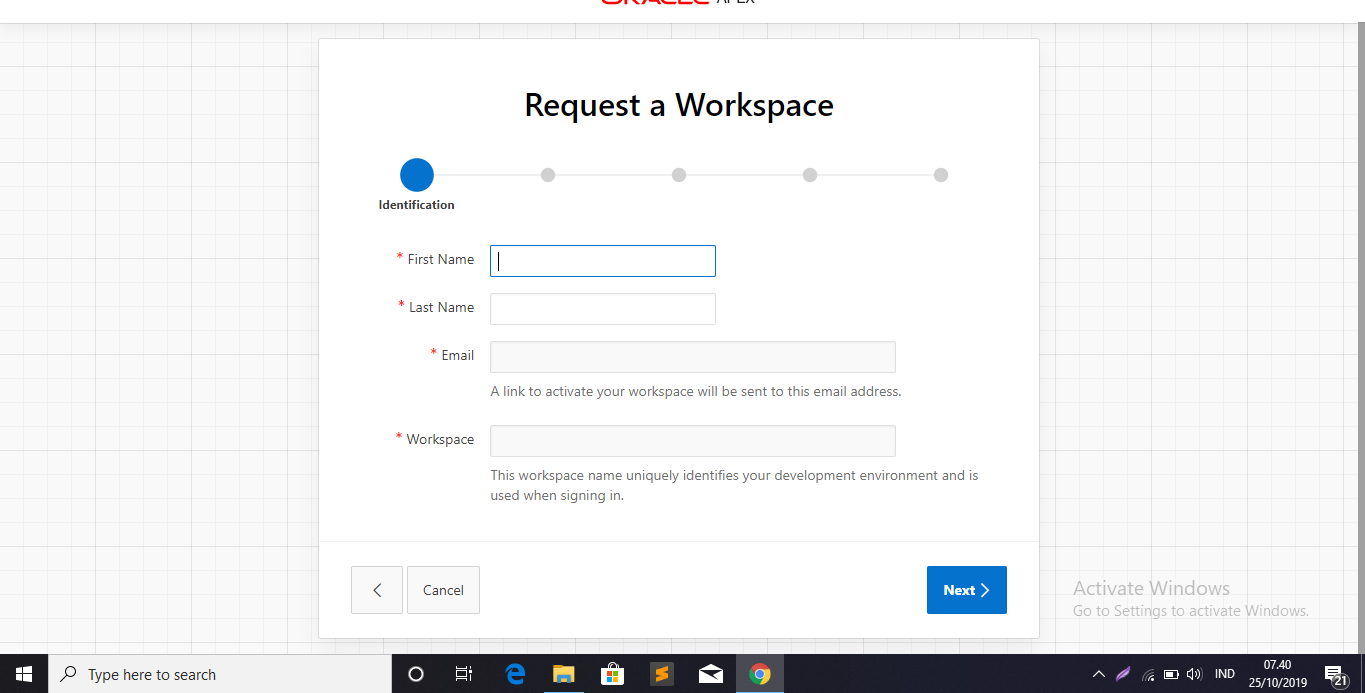
\includegraphics[scale=0.2]{apex/apex2.png}
    \caption{\textit{cara 2}}
    \end{center}

\item[3]Lengkapi data diri dan isi nama unik  untuk workspace.
    \begin{center}
    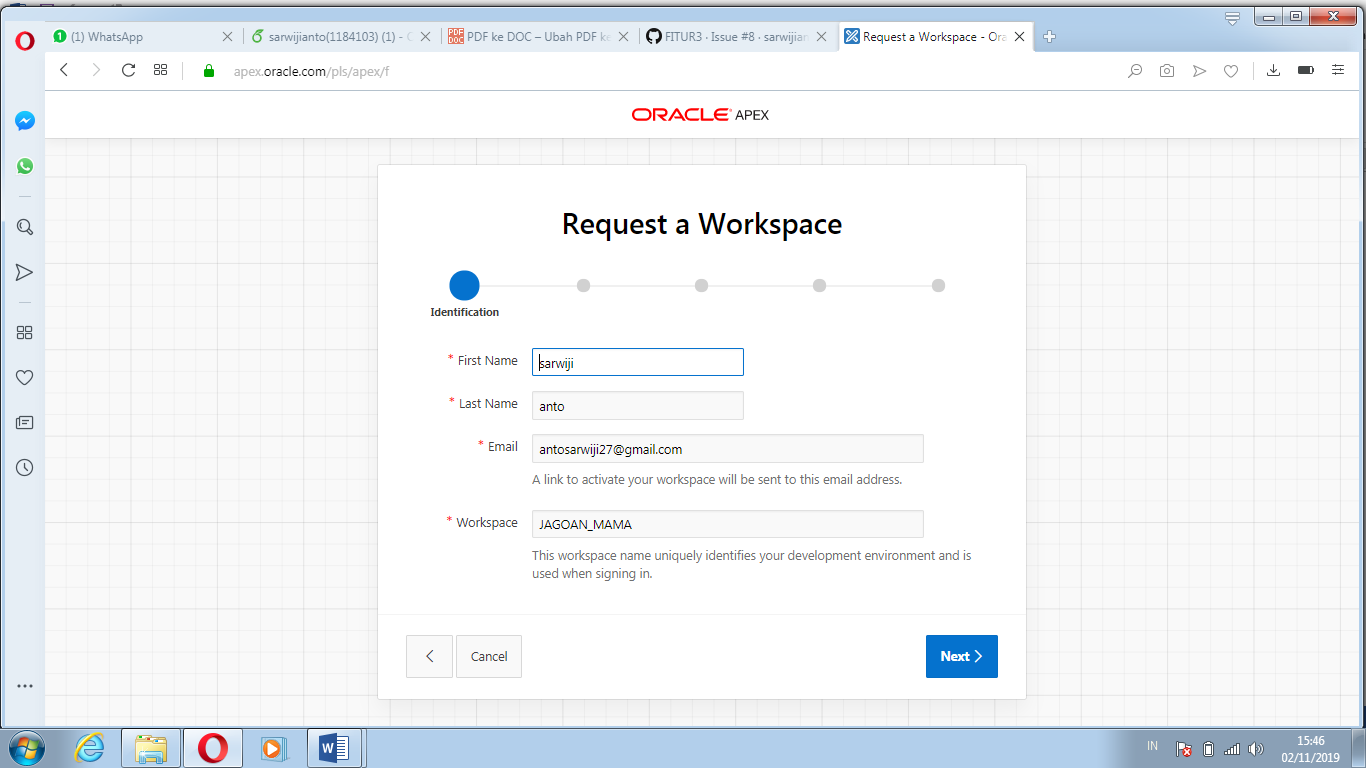
\includegraphics[scale=0.2]{apex/db1.png}
    \caption{\textit{cara 3}}
    \end{center}

        
\item[4]Centang, lalu pilih next.  
    \begin{center}
    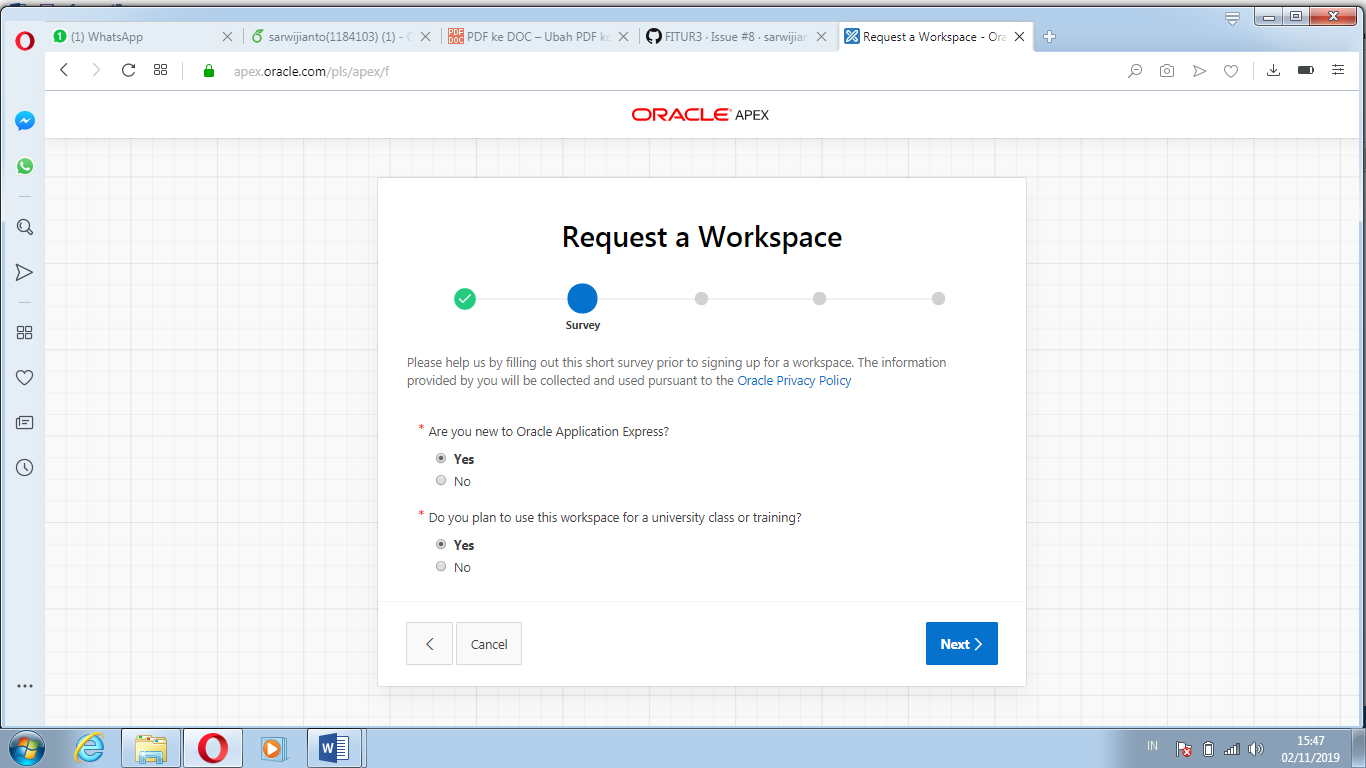
\includegraphics[scale=0.2]{apex/db2.png}
    \caption{\textit{cara 4}}
    \end{center}
      
\item[5]Isi alasan pada kolom alasan merequest workspace, lalu next
    \begin{center}
    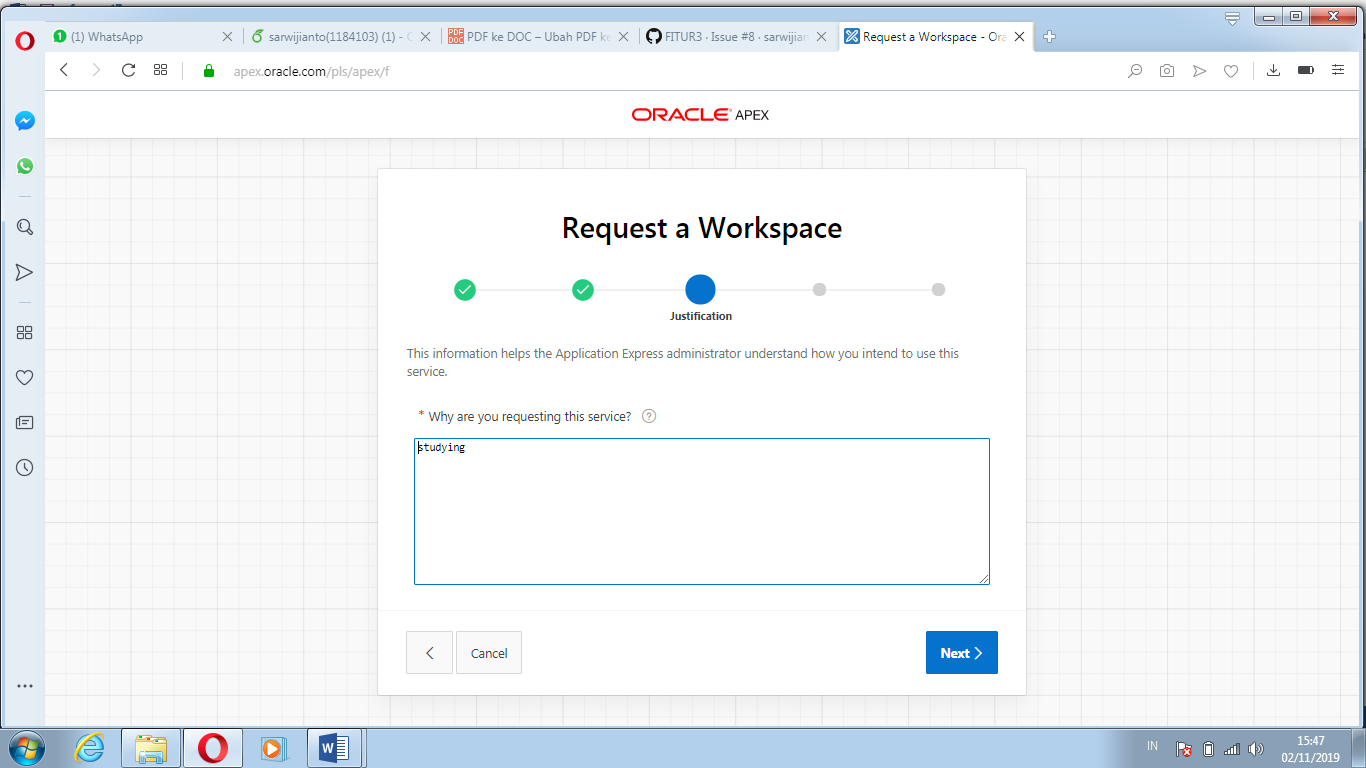
\includegraphics[scale=0.2]{apex/db3.png}
    \caption{\textit{cara 5}}
    \end{center}
 
\item[6] Centang Accept, lalu klik next.
    \begin{center}
    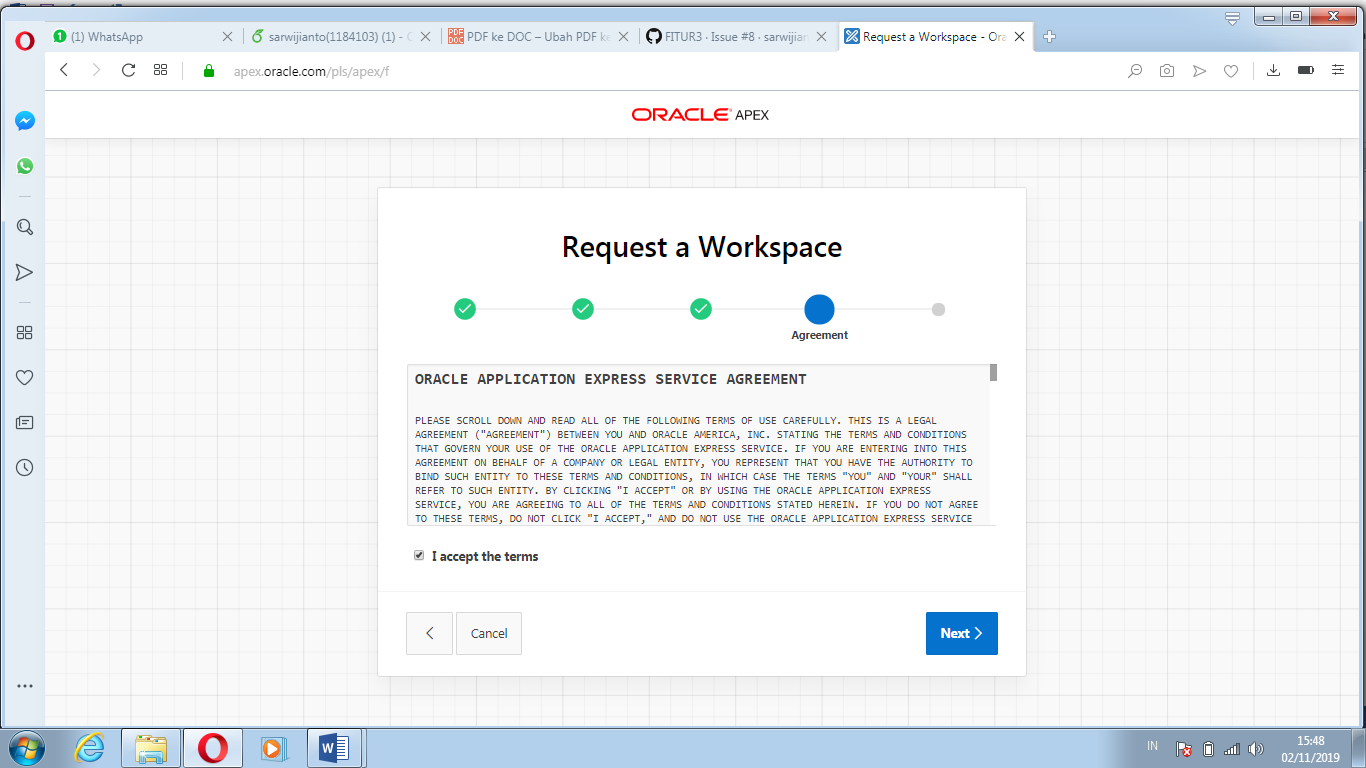
\includegraphics[scale=0.2]{apex/db4.png}
    \caption{\textit{cara 6}}
    \end{center}
    \label{gambar}
    \end{figure}
\begin{figure}
\item[7] Tahapan terakhir untuk mengkonfirmasi apakah ini anda, lalu klik next.
    \begin{center}
    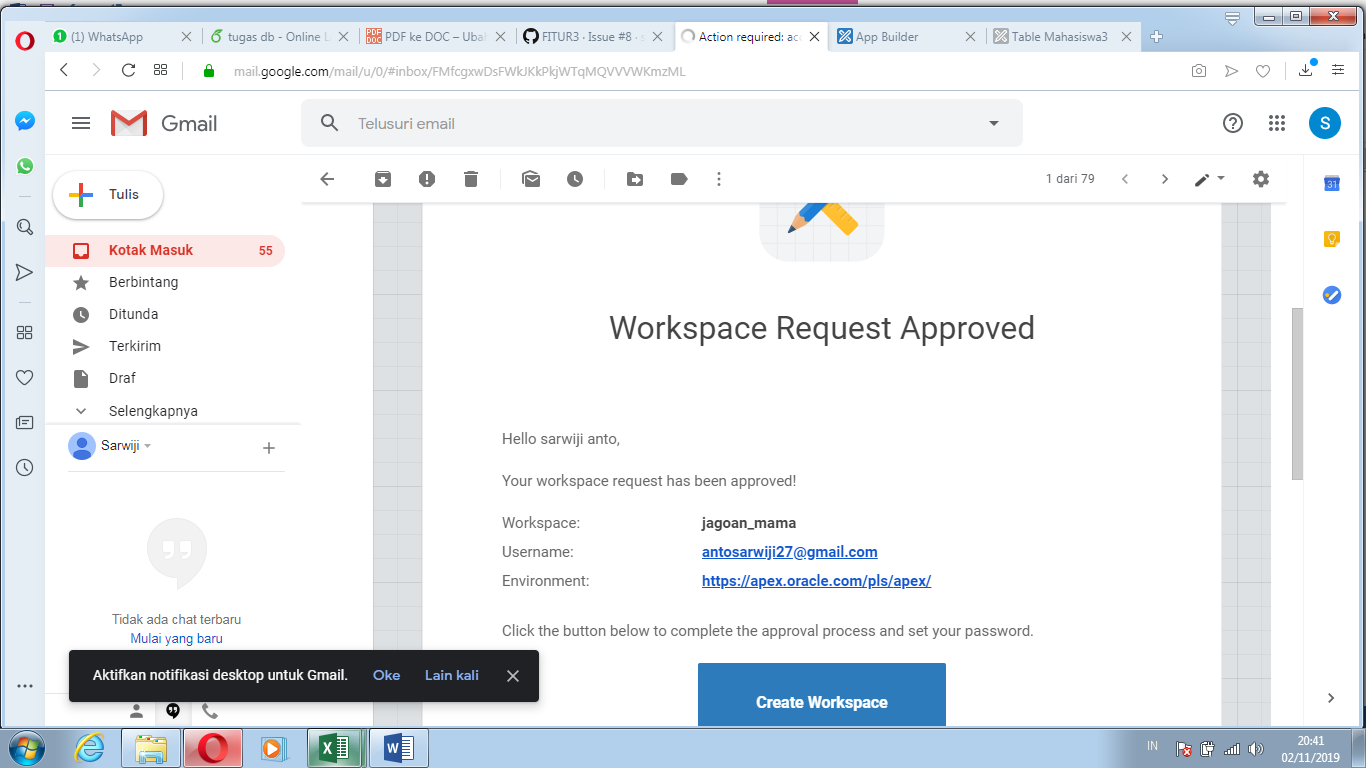
\includegraphics[scale=0.2]{apex/db6.png}
    \caption{\textit{cara 7}}
    \end{center}
    \label{gambar}
    \end{figure}
  \begin{figure}
\item[8] Workspace Sukses Dibuat.

    \begin{center}
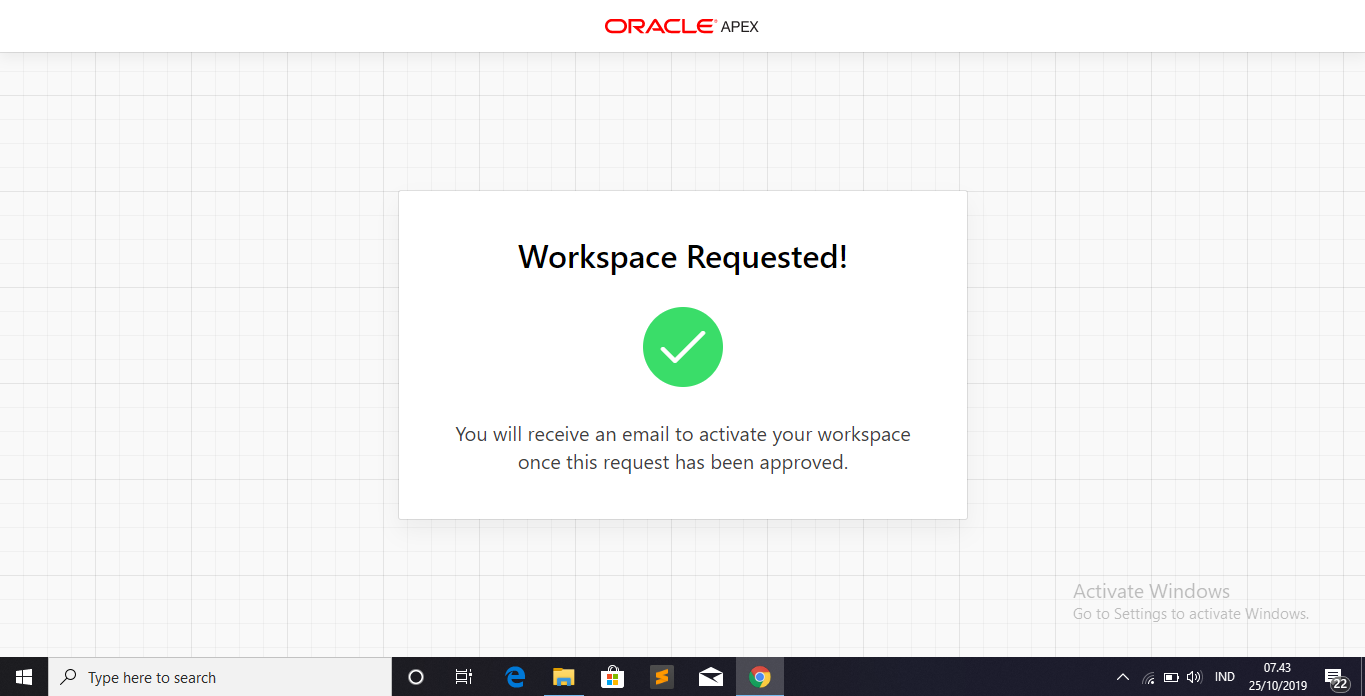
\includegraphics[scale=0.2]{apex/apex3.png}
    \caption{\textit{cara 8}}
        \end{center}
\label{gambar}
\end{figure}

\begin{figure}
\item[9] Email konfirmasi bahwa Workspace yang dibuat telah di Acc.

    \begin{center}
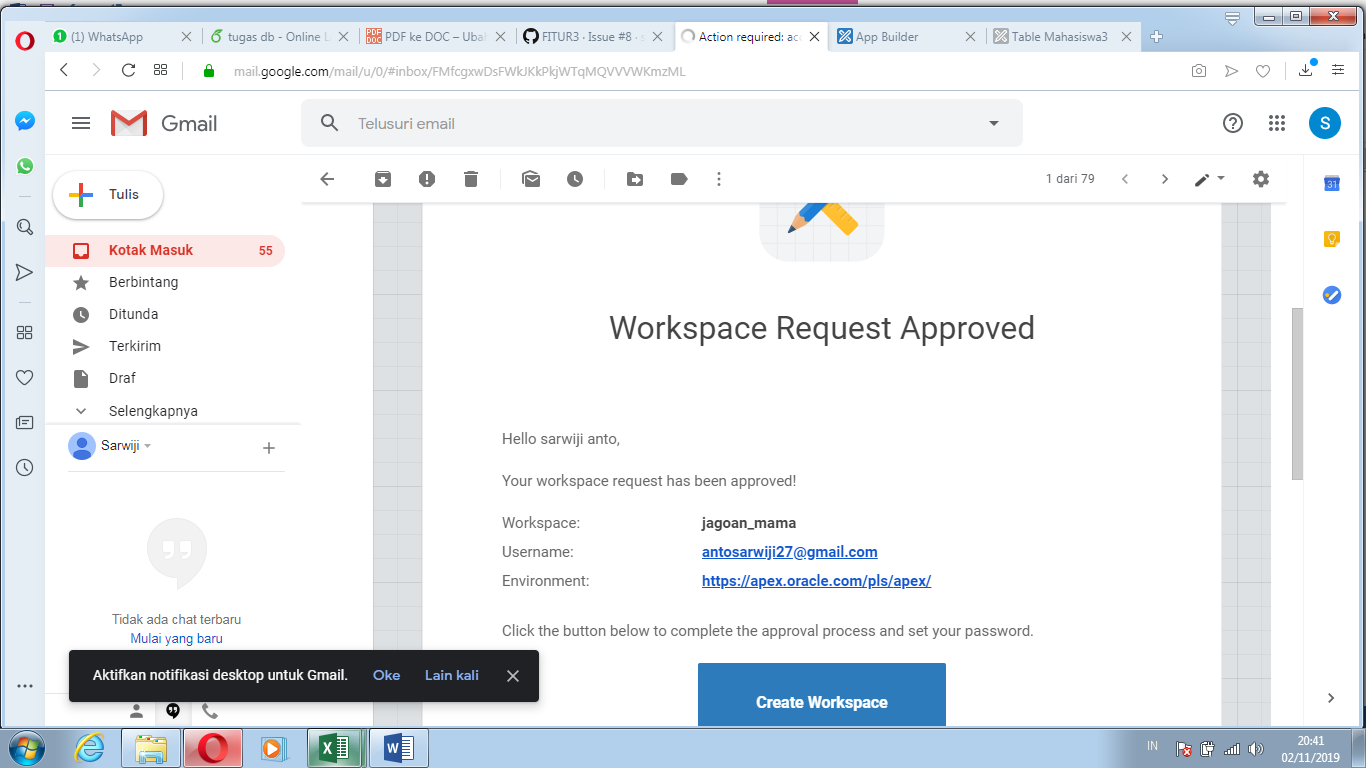
\includegraphics[scale=0.2]{apex/db9.png}
    \caption{\textit{cara9.}}
        \end{center}
\label{gambar}
\end{figure}

\begin{figure}
\item[10] Workspace baru telah dibuat setelah itu lanjutkan dengan pilih create workspace dan isi dengan password baru.

    \begin{center}
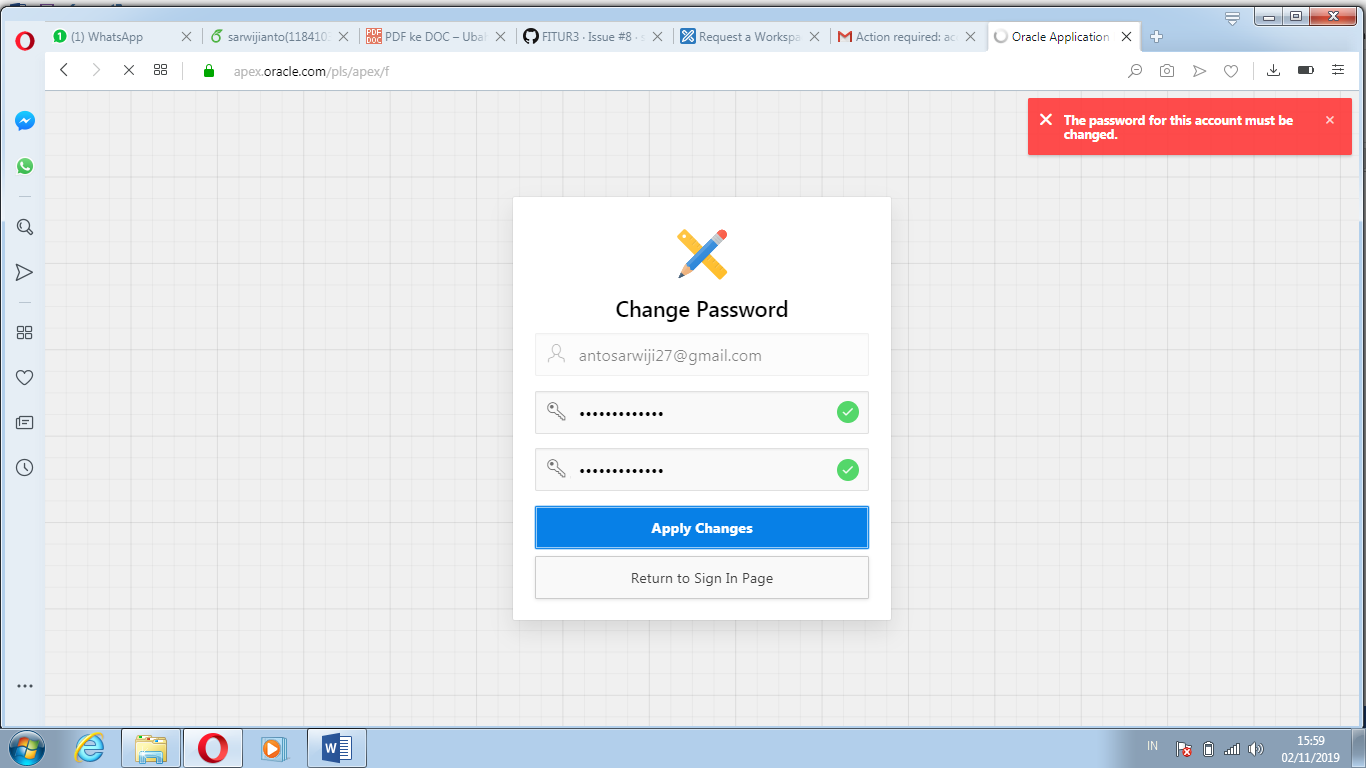
\includegraphics[scale=0.2]{apex/db8.png}
    \caption{\textit{cara 10}}
        \end{center}
\label{gambar}
\end{figure}

\begin{figure}
\item[11] Lakukan Sign in akun workspace yang baru saja di buat.

\end{figure}

\begin{figure}
\item[12] Kita akan masuk ke tampilan awal, langsung pilih app builder.

    
\end{figure}

\begin{figure}
\item[13] dari App Builder lalu klik Create New App.

\end{figure}

\begin{figure}
\item[14] Pilih Copy and Paste, pilih data CSV atau Sample Data Set pilih Project and Tasks.

\end{figure}

\begin{figure}
\item[15] Setelah Sudah me-Load data, tampilan selanjutnya akan seperti berikut. masukkan nama tabel {SPREADSHEET}, setelah itu create Application dan beri nama spreadsheet, kemudian create application.
\
\end{figure}

\begin{figure}
\item[16] klik Create Application .
\begin{center}
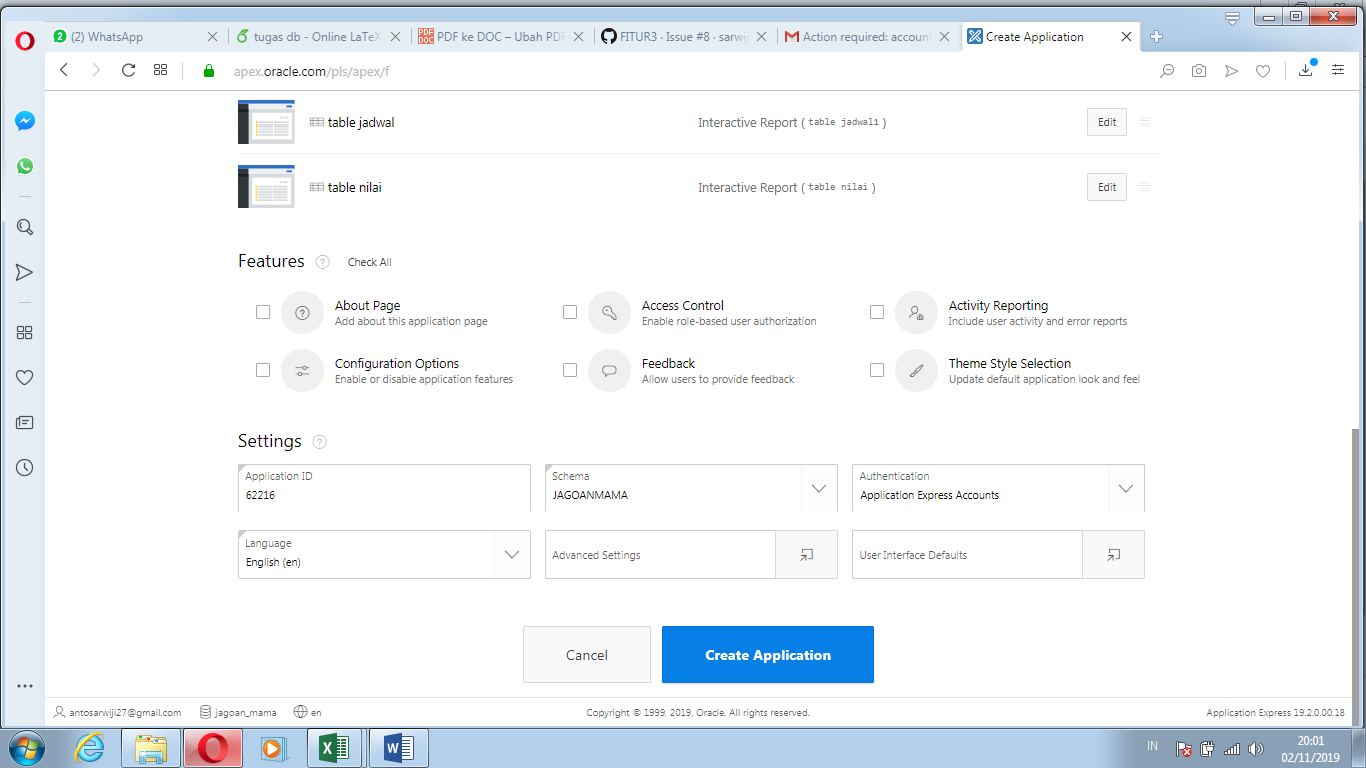
\includegraphics[scale=0.2]{apex/db10.png}
    \caption{\textit{cara 16}}
        \end{center}
\label{gambar}
\end{figure}


\begin{figure}
\item[17]Sekarang kita masuk ke halaman App Builder project Spreadsheet yang telah berhasil dibuat. aplikasi yang baru dibuat akan tampil di halaman designer, setelah itu klik Run application .
\end{figure}
\begin{center}
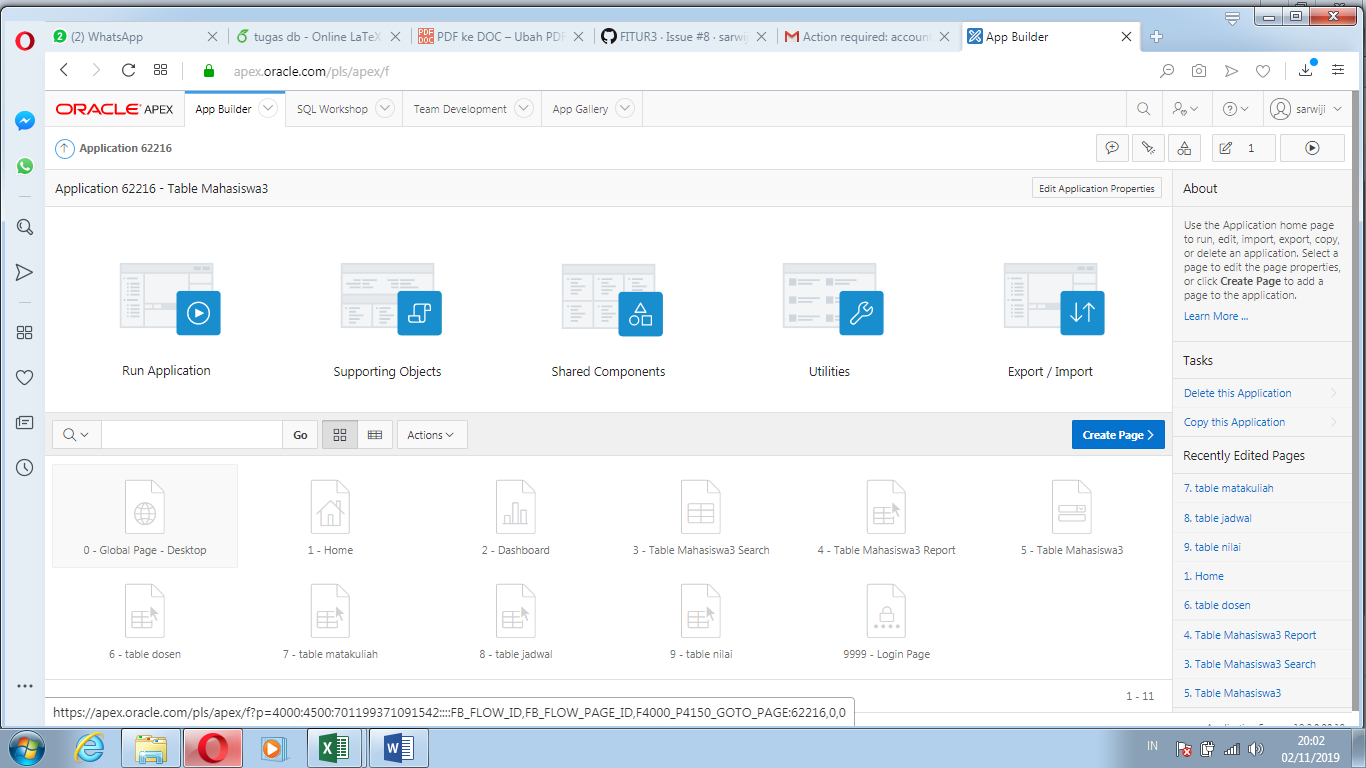
\includegraphics[scale=0.2]{apex/db11.png}
    \caption{\textit{cara 17}}
        \end{center}
\label{gambar}
\begin{figure}
\item[18]Login ke Aplikasi Oracle APEX .

      \begin{center}
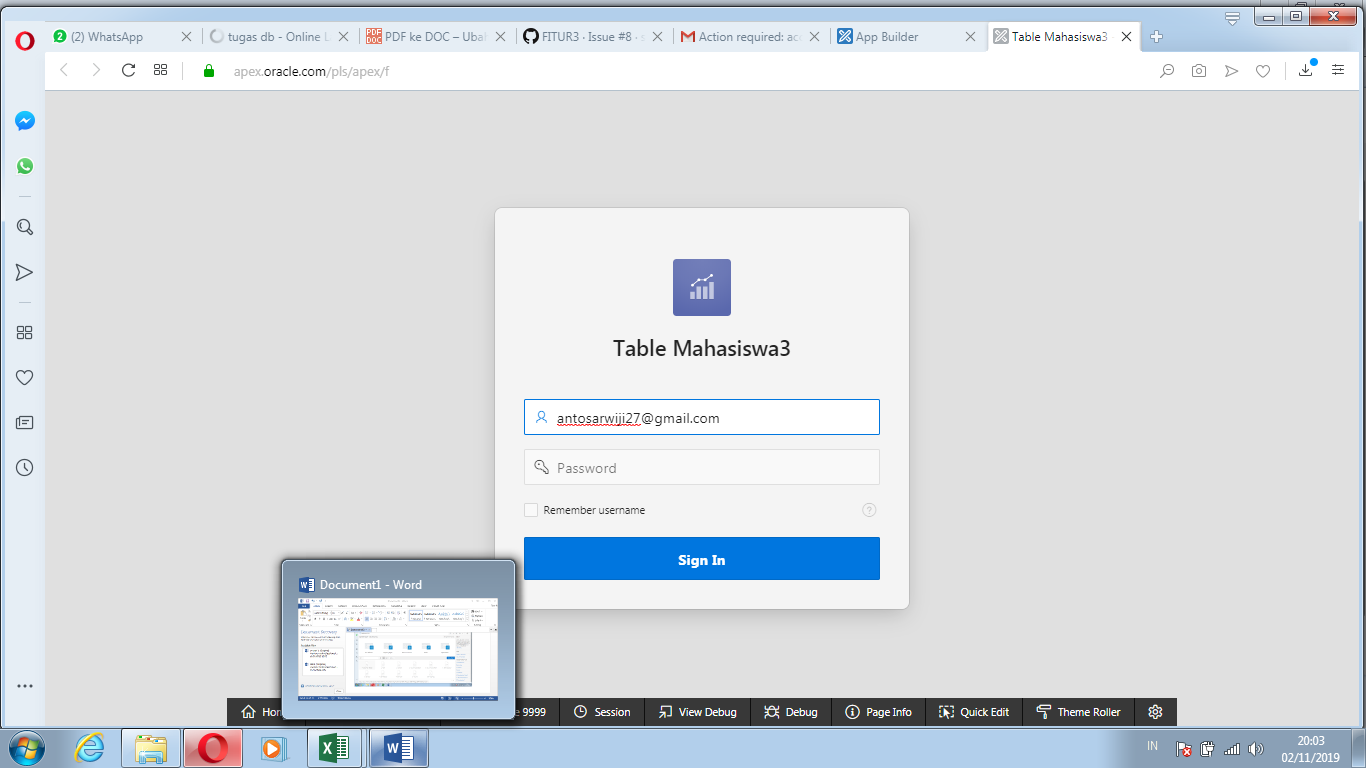
\includegraphics[scale=0.2]{apex/db12.png}
    \caption{\textit{cara 18}}
        \end{center}
\label{gambar}
\end{figure}

\begin{figure}
\item[19]Sekarang aplikasi Oracle Apex sudah dijalankan.

    \begin{center}
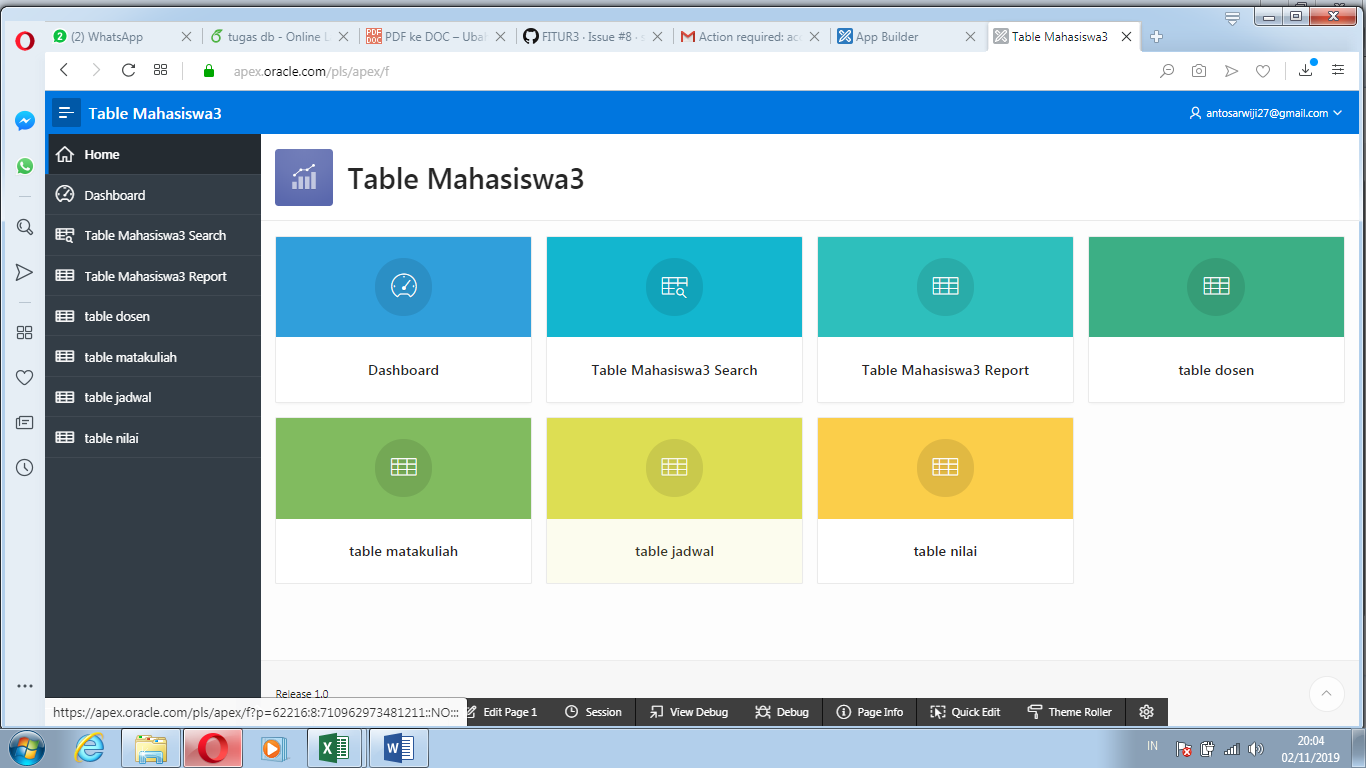
\includegraphics[scale=0.2]{apex/db13.png}
    \caption{\textit{Masuk ke Aplikasi}}
        \end{center}
\label{gambar}
\end{figure}
\newpage
\paragraph{Email}
username:antosarwiji@gmail.com\\
password:sarwiji123456\\
https://apex.oracle.com/pls/apex/f?p=62216:1:701199371091542:::::\\

\end{enumerate}
\end{document}